\documentclass[14pt]{extbook}
\usepackage{multicol, enumerate, enumitem, hyperref, color, soul, setspace, parskip, fancyhdr} %General Packages
\usepackage{amssymb, amsthm, amsmath, bbm, latexsym, units, mathtools} %Math Packages
\everymath{\displaystyle} %All math in Display Style
% Packages with additional options
\usepackage[headsep=0.5cm,headheight=12pt, left=1 in,right= 1 in,top= 1 in,bottom= 1 in]{geometry}
\usepackage[usenames,dvipsnames]{xcolor}
\usepackage{dashrule}  % Package to use the command below to create lines between items
\newcommand{\litem}[1]{\item#1\hspace*{-1cm}\rule{\textwidth}{0.4pt}}
\pagestyle{fancy}
\lhead{Progress Quiz 4}
\chead{}
\rhead{Version B}
\lfoot{4378-7085}
\cfoot{}
\rfoot{Fall 2020}
\begin{document}

\begin{enumerate}
\litem{
Write the equation of the graph presented below in the form $f(x)=ax^2+bx+c$, assuming  $a=1$ or $a=-1$. Then, choose the intervals that $a, b,$ and $c$ belong to.
\begin{center}
    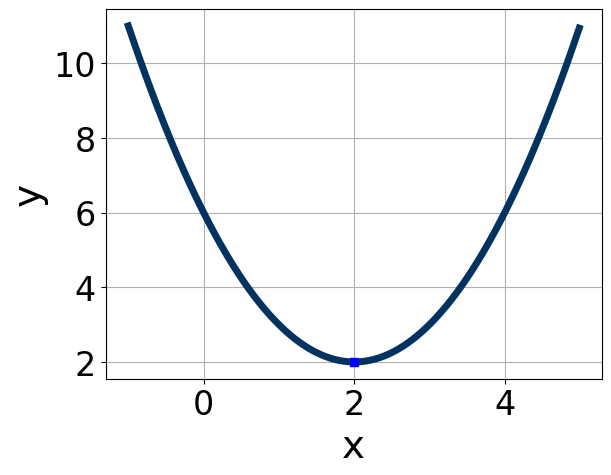
\includegraphics[width=0.5\textwidth]{../Figures/quadraticGraphToEquationCopyB.png}
\end{center}
\begin{enumerate}[label=\Alph*.]
\item \( a \in [-0.1, 1.4], \hspace*{5mm} b \in [8, 9], \text{ and } \hspace*{5mm} c \in [21, 23] \)
\item \( a \in [-2.9, 0.7], \hspace*{5mm} b \in [-8, -6], \text{ and } \hspace*{5mm} c \in [-24, -19] \)
\item \( a \in [-2.9, 0.7], \hspace*{5mm} b \in [8, 9], \text{ and } \hspace*{5mm} c \in [-10, -8] \)
\item \( a \in [-0.1, 1.4], \hspace*{5mm} b \in [-8, -6], \text{ and } \hspace*{5mm} c \in [21, 23] \)
\item \( a \in [-2.9, 0.7], \hspace*{5mm} b \in [-8, -6], \text{ and } \hspace*{5mm} c \in [-10, -8] \)

\end{enumerate} }
\litem{
Solve the quadratic equation below. Then, choose the intervals that the solutions $x_1$ and $x_2$ belong to, with $x_1 \leq x_2$.\[ 25x^{2} -60 x + 36 = 0 \]\begin{enumerate}[label=\Alph*.]
\item \( x_1 \in [0.56, 0.63] \text{ and } x_2 \in [2.23, 3.2] \)
\item \( x_1 \in [0.33, 0.41] \text{ and } x_2 \in [2.54, 4.31] \)
\item \( x_1 \in [29.96, 30.07] \text{ and } x_2 \in [28.73, 32.35] \)
\item \( x_1 \in [0.13, 0.26] \text{ and } x_2 \in [5.97, 6.7] \)
\item \( x_1 \in [1.18, 1.29] \text{ and } x_2 \in [0.24, 1.5] \)

\end{enumerate} }
\litem{
Factor the quadratic below. Then, choose the intervals that contain the constants in the form $(ax+b)(cx+d); b \leq d.$\[ 24x^{2} +2 x -15 \]\begin{enumerate}[label=\Alph*.]
\item \( a \in [1.78, 2.82], \hspace*{5mm} b \in [-4, -1], \hspace*{5mm} c \in [10.5, 13.9], \text{ and } \hspace*{5mm} d \in [0, 9] \)
\item \( a \in [0.66, 1.4], \hspace*{5mm} b \in [-23, -15], \hspace*{5mm} c \in [0.8, 2], \text{ and } \hspace*{5mm} d \in [18, 21] \)
\item \( a \in [3.71, 4.51], \hspace*{5mm} b \in [-4, -1], \hspace*{5mm} c \in [5.5, 8.1], \text{ and } \hspace*{5mm} d \in [0, 9] \)
\item \( a \in [7.19, 8.07], \hspace*{5mm} b \in [-4, -1], \hspace*{5mm} c \in [2.6, 5.1], \text{ and } \hspace*{5mm} d \in [0, 9] \)
\item \( \text{None of the above.} \)

\end{enumerate} }
\litem{
Solve the quadratic equation below. Then, choose the intervals that the solutions belong to, with $x_1 \leq x_2$ (if they exist).\[ -10x^{2} +7 x + 4 = 0 \]\begin{enumerate}[label=\Alph*.]
\item \( x_1 \in [-14.26, -14] \text{ and } x_2 \in [13.83, 15.02] \)
\item \( x_1 \in [-1.01, 0.64] \text{ and } x_2 \in [0.41, 1.63] \)
\item \( x_1 \in [-11.14, -10.21] \text{ and } x_2 \in [2.94, 4.12] \)
\item \( x_1 \in [-1.16, -0.73] \text{ and } x_2 \in [-0.44, 0.93] \)
\item \( \text{There are no Real solutions.} \)

\end{enumerate} }
\litem{
Write the equation of the graph presented below in the form $f(x)=ax^2+bx+c$, assuming  $a=1$ or $a=-1$. Then, choose the intervals that $a, b,$ and $c$ belong to.
\begin{center}
    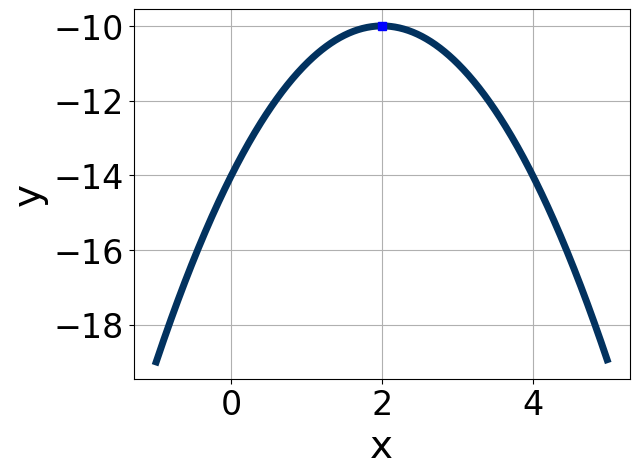
\includegraphics[width=0.5\textwidth]{../Figures/quadraticGraphToEquationB.png}
\end{center}
\begin{enumerate}[label=\Alph*.]
\item \( a \in [-1.2, -0.4], \hspace*{5mm} b \in [-11, -6], \text{ and } \hspace*{5mm} c \in [-18, -16] \)
\item \( a \in [-1.2, -0.4], \hspace*{5mm} b \in [4, 11], \text{ and } \hspace*{5mm} c \in [-18, -16] \)
\item \( a \in [-1.2, -0.4], \hspace*{5mm} b \in [-11, -6], \text{ and } \hspace*{5mm} c \in [-17, -10] \)
\item \( a \in [0.4, 3.1], \hspace*{5mm} b \in [-11, -6], \text{ and } \hspace*{5mm} c \in [13, 18] \)
\item \( a \in [0.4, 3.1], \hspace*{5mm} b \in [4, 11], \text{ and } \hspace*{5mm} c \in [13, 18] \)

\end{enumerate} }
\litem{
Graph the equation below.\[ f(x) = (x-4)^2 - 14 \]\begin{enumerate}[label=\Alph*.]
\begin{multicols}{2}\item 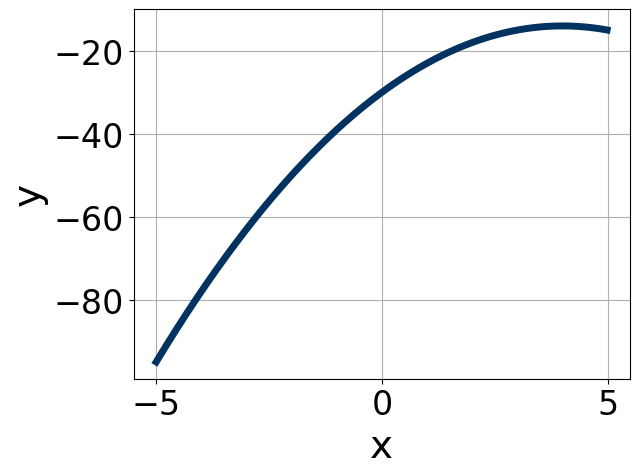
\includegraphics[width = 0.3\textwidth]{../Figures/quadraticEquationToGraphCopyAB.png}\item 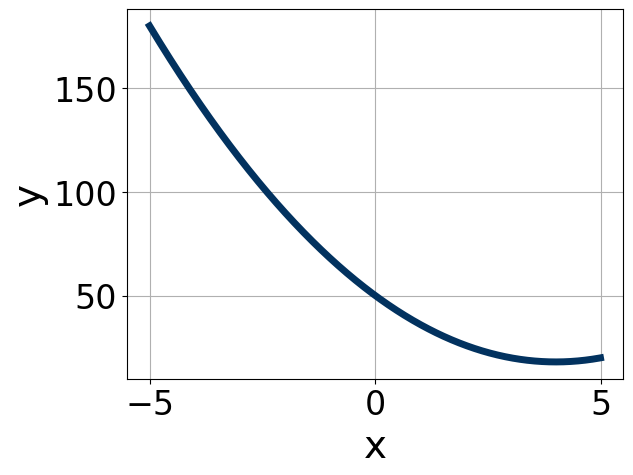
\includegraphics[width = 0.3\textwidth]{../Figures/quadraticEquationToGraphCopyBB.png}\item 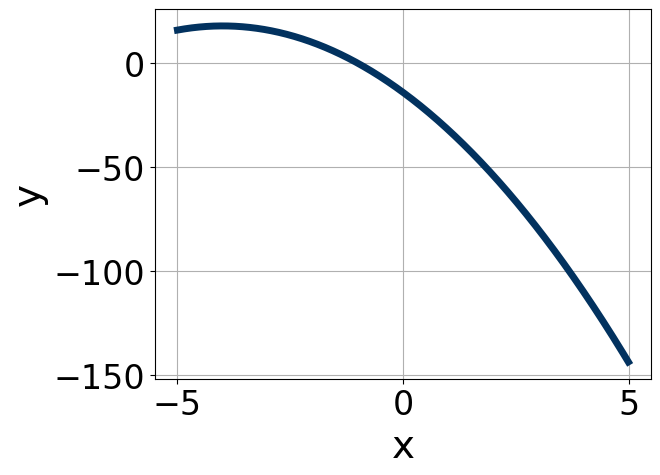
\includegraphics[width = 0.3\textwidth]{../Figures/quadraticEquationToGraphCopyCB.png}\item 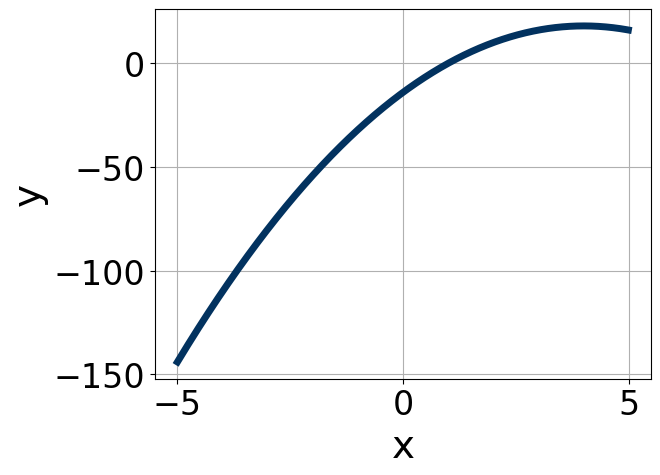
\includegraphics[width = 0.3\textwidth]{../Figures/quadraticEquationToGraphCopyDB.png}\end{multicols}\item None of the above.
\end{enumerate} }
\litem{
Factor the quadratic below. Then, choose the intervals that contain the constants in the form $(ax+b)(cx+d); b \leq d.$\[ 36x^{2} +60 x + 25 \]\begin{enumerate}[label=\Alph*.]
\item \( a \in [0.13, 1.53], \hspace*{5mm} b \in [29, 31], \hspace*{5mm} c \in [-2.5, 2.6], \text{ and } \hspace*{5mm} d \in [29, 32] \)
\item \( a \in [11.83, 12.98], \hspace*{5mm} b \in [3, 9], \hspace*{5mm} c \in [1.7, 4.4], \text{ and } \hspace*{5mm} d \in [2, 8] \)
\item \( a \in [1.64, 3], \hspace*{5mm} b \in [3, 9], \hspace*{5mm} c \in [17, 18.7], \text{ and } \hspace*{5mm} d \in [2, 8] \)
\item \( a \in [4.12, 6.04], \hspace*{5mm} b \in [3, 9], \hspace*{5mm} c \in [4.7, 6.6], \text{ and } \hspace*{5mm} d \in [2, 8] \)
\item \( \text{None of the above.} \)

\end{enumerate} }
\litem{
Solve the quadratic equation below. Then, choose the intervals that the solutions $x_1$ and $x_2$ belong to, with $x_1 \leq x_2$.\[ 10x^{2} -57 x + 54 = 0 \]\begin{enumerate}[label=\Alph*.]
\item \( x_1 \in [2.17, 2.28] \text{ and } x_2 \in [1.72, 2.57] \)
\item \( x_1 \in [0.87, 0.9] \text{ and } x_2 \in [5.77, 6.44] \)
\item \( x_1 \in [0.13, 0.51] \text{ and } x_2 \in [12.77, 13.61] \)
\item \( x_1 \in [11.65, 12.12] \text{ and } x_2 \in [44.77, 45.15] \)
\item \( x_1 \in [1.19, 1.35] \text{ and } x_2 \in [4.06, 4.61] \)

\end{enumerate} }
\litem{
Solve the quadratic equation below. Then, choose the intervals that the solutions belong to, with $x_1 \leq x_2$ (if they exist).\[ 20x^{2} +7 x -2 = 0 \]\begin{enumerate}[label=\Alph*.]
\item \( x_1 \in [-10.9, -10.2] \text{ and } x_2 \in [3.67, 3.98] \)
\item \( x_1 \in [-15.2, -14.1] \text{ and } x_2 \in [14.18, 14.73] \)
\item \( x_1 \in [-0.3, 0.2] \text{ and } x_2 \in [0.45, 0.84] \)
\item \( x_1 \in [-2, -0.3] \text{ and } x_2 \in [-0.21, 0.24] \)
\item \( \text{There are no Real solutions.} \)

\end{enumerate} }
\litem{
Graph the equation below.\[ f(x) = -(x+1)^2 - 13 \]\begin{enumerate}[label=\Alph*.]
\begin{multicols}{2}\item 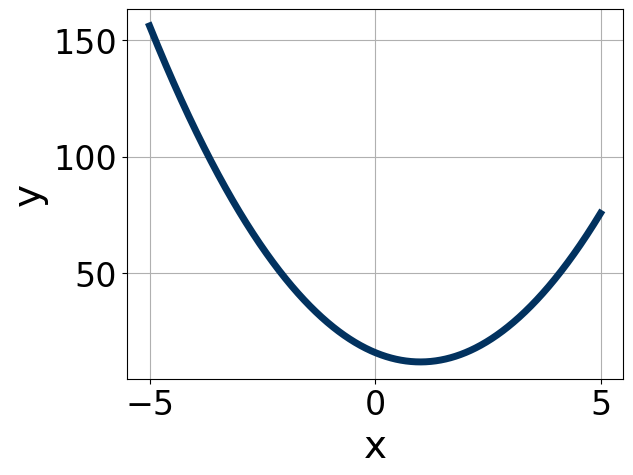
\includegraphics[width = 0.3\textwidth]{../Figures/quadraticEquationToGraphAB.png}\item 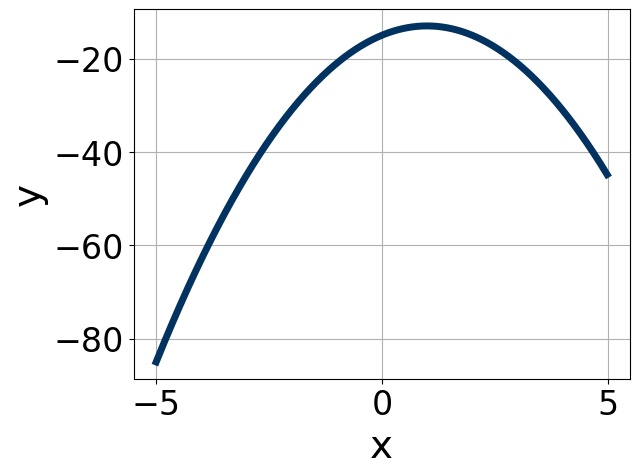
\includegraphics[width = 0.3\textwidth]{../Figures/quadraticEquationToGraphBB.png}\item 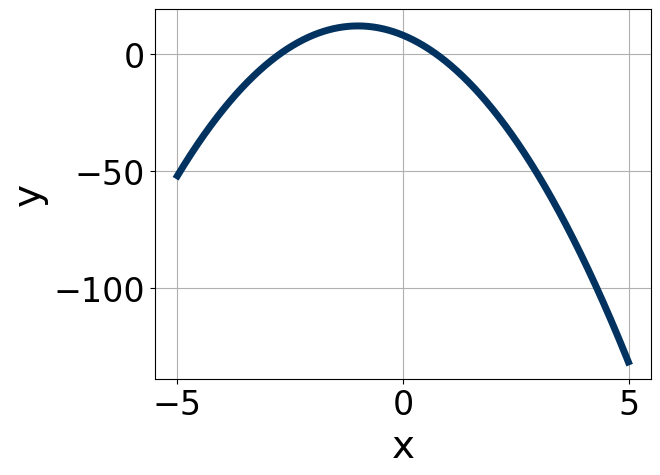
\includegraphics[width = 0.3\textwidth]{../Figures/quadraticEquationToGraphCB.png}\item 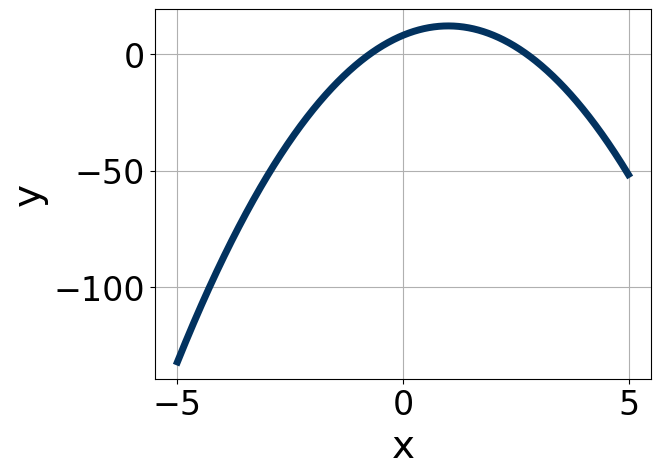
\includegraphics[width = 0.3\textwidth]{../Figures/quadraticEquationToGraphDB.png}\end{multicols}\item None of the above.
\end{enumerate} }
\end{enumerate}

\end{document}